\documentclass{beamer}

\usepackage{epsfig}
\usepackage{multicol}
\usepackage{geometry}
%\usepackage[dvipsnames]{xcolor}
\usepackage{textcomp}
\usepackage{graphicx}
\usepackage{caption}
\usepackage{subcaption}
\usepackage{amsmath}
\usepackage{tcolorbox}
\usetheme{Boadilla}
\usepackage{pict2e}
\usepackage{tikz}
\usepackage{xcolor}


\title[Traitement du signal numérique]{Traitement du signal numérique - HEI4 IMS}
\author[Antony Bazir]{}

\setlength{\unitlength}{1cm}

\begin{document}


\section{Filtres numériques: Synthèses et mise en oeuvre}
\subsection{Introduction}
\begin{frame}
\frametitle{Introduction}
Dans la section précédente on a étudie un filtre récursif et un filtre non récursif \\
\vspace{0.3cm}

\begin{columns}

\column{60mm}
\only<2->{
\begin{center}
	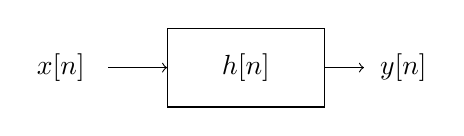
\begin{tikzpicture}
	\draw (2.15,0) node {$x[n]$};
	
	\draw[->] (2.75,0)-- (3.5,0);
	\draw (3.5,-0.5) rectangle(5.5,0.5) ;
	\draw (4.5,0) node {$h[n]$};
	
	\draw[->] (5.5,0)-- (6,0);

	\draw (6.5,0) node {$y[n]$};
	%\draw (4.5,-2) node {filtre non-récursif};
\end{tikzpicture}
\end{center}
}

\column{60mm}
\only<2->{
\begin{center}
	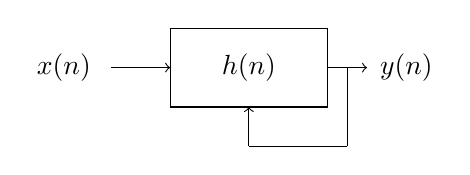
\begin{tikzpicture}
	\draw (2.15,0) node {$x(n)$};

	
	\draw[->] (2.75,0)-- (3.5,0);
	\draw (3.5,-0.5) rectangle(5.5,0.5) ;
	\draw (4.5,0) node {$h(n)$};
	
	\draw[->] (5.5,0)-- (6,0); 
	\draw (6.5,0) node {$y(n)$};

	%\draw (4.5,-2) node {filtre récursif};
	
	\draw[-] (5.75,0)-- (5.75,-1);
	\draw[-] (5.75,-1)-- (4.5,-1);
	\draw[->] (4.5,-1)-- (4.5,-0.5);
	\end{tikzpicture}
\end{center}

}

\end{columns}
%\phantom{.\\}
\vspace{1.3cm}
\only<3->{
On a étudié les propriétés de filtres existants mais on ne sait pas comment les "fabriquer" \only<4->{$\rightarrow$ Synthèse de filtre}
}

\end{frame}


\begin{frame}
\frametitle{Introduction}
Les méthodes de synthèse pour les filtres récursifs et non récursifs sont assez différentes...\\
\vspace{0.3cm}

\begin{columns}

\column{60mm}
\begin{center}
	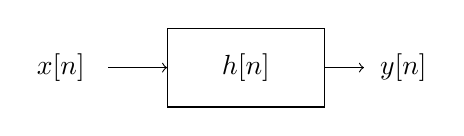
\begin{tikzpicture}
	\draw (2.15,0) node {$x[n]$};
	
	\draw[->] (2.75,0)-- (3.5,0);
	\draw (3.5,-0.5) rectangle(5.5,0.5) ;
	\draw (4.5,0) node {$h[n]$};
	
	\draw[->] (5.5,0)-- (6,0);

	\draw (6.5,0) node {$y[n]$};
	%\draw (4.5,-2) node {filtre non-récursif};
\end{tikzpicture}
\end{center}
\only<2->{
Objectif : calculer les \textbf{coefficients de la réponse impulsionnelles} qui correspondent au gabarit
}

\column{60mm}
\begin{center}
	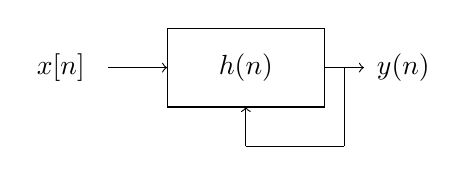
\begin{tikzpicture}
	\draw (2.15,0) node {$x[n]$};

	
	\draw[->] (2.75,0)-- (3.5,0);
	\draw (3.5,-0.5) rectangle(5.5,0.5) ;
	\draw (4.5,0) node {$h(n)$};
	
	\draw[->] (5.5,0)-- (6,0); 
	\draw (6.5,0) node {$y(n)$};

	%\draw (4.5,-2) node {filtre récursif};
	
	\draw[-] (5.75,0)-- (5.75,-1);
	\draw[-] (5.75,-1)-- (4.5,-1);
	\draw[->] (4.5,-1)-- (4.5,-0.5);
	\end{tikzpicture}
\end{center}

\only<2->{
Objectif : \textbf{discrétiser un filtre continu} qui corresponde au gabarit
}

\end{columns}
\end{frame}

\subsection{Synthèse de filtres non-récursifs:  \'Etude filtre passe-bas idéal}
\subsubsection{Réponse impulsionnelle idéale}
\begin{frame}
On commence par les \textbf{filtres non-récursifs}\\
\frametitle{Premier exemple :  Filtre passe-bas idéal}

\vspace{0.3cm}
synthèse de filtre : Passe-bas idéal\\
\vspace{0.3cm}
\begin{columns}

\column{60mm}
\begin{center}
\begin{tikzpicture}

	\draw[->] (-0.5,0)-- (3.5,0);
\draw (-0.3,-0.3) node {0};
\draw[->] (0,0)-- (0,3);
\draw (3.6,0.25) node {$f$};
\draw (0,3.5) node {$|H(f)|$};
\only<1>{
\draw (1,-0.3) node {$f_1$};
\draw (2,-0.3) node {$f_2$};
\draw (-0.6,1.7) node {$1 - \delta_1$};
\draw (-0.6,2.3) node {$1 + \delta_1$};
\draw (-0.3,0.3) node {$\delta_2$};
}
\draw (3,-0.3) node {$f_e/2$};

\only<1>{
\draw[thick,blue](0,1.7)--(1,1.7)--(1,0);
\draw[thick,blue](0,2.3)--(1,2.3)--(1,3);
\draw[thick,blue](2,3)--(2,0.3)--(3,0.3);
}

\only<2->{
\draw[dashed,blue](0,1.7)--(1,1.7)--(1,0);
\draw[dashed,blue](0,2.3)--(1,2.3)--(1,3);
\draw[dashed,blue](2,3)--(2,0.3)--(3,0.3);
}

\only<2->{
	\draw[thick,red]   (0,2)--(1.5,2)--(1.5,0)--(3,0);
	\draw (1.5,-0.3) node {$f_e/4$};
}

\end{tikzpicture}
\end{center}

\column{60mm}
\only<3->{
Ce filtre va correspondre à une réponse impulsionnelle...\\
\vspace{0.5cm}
Comment l'obtenir ?

\begin{itemize} 
\item<4-> Transformée en Z inverse ? \only<5->{ Non... Trop compliqué} 
\item<6-> Développer en série de Fourier
\item<7-> Calculer la fonction continue connue et échantillonner
\end{itemize} 

}

\end{columns}

\end{frame}


\begin{frame}
\frametitle{Premier exemple :  Filtre passe-bas idéal}

\vspace{0.3cm}
Pour comprendre les défis de la synthèse de filtre : Passe-bas idéal\\
\vspace{0.3cm}
\begin{columns}

\column{60mm}
\begin{center}
\begin{tikzpicture}

	\draw[->] (-0.5,0)-- (3.5,0);
\draw (-0.3,-0.3) node {0};
\draw[->] (0,0)-- (0,3);
\draw (3.6,0.25) node {$f$};
\draw (0,3.5) node {$|H(f)|$};

\draw (3,-0.3) node {$f_e/2$};


\draw[dashed,blue](0,1.7)--(1,1.7)--(1,0);
\draw[dashed,blue](0,2.3)--(1,2.3)--(1,3);
\draw[dashed,blue](2,3)--(2,0.3)--(3,0.3);

	\draw[thick,red]   (0,2)--(1.5,2)--(1.5,0)--(3,0);
	\draw (1.5,-0.3) node {$f_e/4$};

\end{tikzpicture}
\end{center}

\column{60mm}
Développement en série de Fourier ? \\
\vspace{0.1cm}
\begin{itemize}
\item<2-> Spectre jusqu'à $f_e/2$ $\rightarrow$ signal discret
\vspace{0.1cm}
\item<3-> Signal discret  $f_e/2$ $\rightarrow$ spectre périodique
\vspace{0.1cm}
\item<4-> Spectre périodique  $f_e/2$ $\rightarrow$ spectre développable en série de fourier 
\vspace{0.1cm}
\item<5-> Coefficients de fourier d'une fct°  $f_e/2$ $\rightarrow$ réponse impulsionnelle discrète...
\end{itemize}

\end{columns}

\end{frame}

\begin{frame}
\frametitle{Premier exemple :  Filtre passe-bas idéal}


\vspace{0.3cm}
Pour comprendre les défis de la synthèse de filtre : Passe-bas idéal\\
\vspace{0.3cm}
\begin{columns}

\column{60mm}
\begin{center}
\begin{tikzpicture}

	\draw[->] (-0.5,0)-- (3.5,0);
\draw (-0.3,-0.3) node {0};
\draw[->] (0,0)-- (0,3);
\draw (3.6,0.25) node {$f$};
\draw (0,3.5) node {$|H(f)|$};

\draw (3,-0.3) node {$f_e/2$};


\draw[dashed,blue](0,1.7)--(1,1.7)--(1,0);
\draw[dashed,blue](0,2.3)--(1,2.3)--(1,3);
\draw[dashed,blue](2,3)--(2,0.3)--(3,0.3);

	\draw[thick,red]   (0,2)--(1.5,2)--(1.5,0)--(3,0);
	\draw (1.5,-0.3) node {$f_e/4$};

\end{tikzpicture}
\end{center}

\column{60mm}
Réponse impulsionnelle continue + échantillonnage ? \\
\vspace{0.1cm}
\begin{itemize}
\item<2-> Spectre jusqu'à $f_e/2$ $\rightarrow$ Spectre jusqu'à $+ \infty$
\vspace{0.1cm}
\item<3-> TF inverse sur spectre $\rightarrow$ Signal temporel continu 
\vspace{0.1cm}
\item<4-> Signal temporel continu  $\rightarrow$ Signal échantillonné à $f_e$
\vspace{0.1cm}
\end{itemize}

\end{columns}
\end{frame}

\begin{frame}
\frametitle{Premier exemple :  Filtre passe-bas idéal}
Résultat des 3 méthodes:\\
\vspace{0.3cm}
\begin{columns}

\column{60mm}
Réponse en fréquence :\\
\vspace{0.2cm}
\begin{center}
\begin{tikzpicture}

	\draw[->] (-0.5,0)-- (3.5,0);
\draw (-0.3,-0.3) node {0};
\draw[->] (0,0)-- (0,3);
\draw (3.6,0.25) node {$f$};
\draw (0,3.5) node {$|H(f)|$};

\draw (3,-0.3) node {$f_e/2$};


\draw[dashed,blue](0,1.7)--(1,1.7)--(1,0);
\draw[dashed,blue](0,2.3)--(1,2.3)--(1,3);
\draw[dashed,blue](2,3)--(2,0.3)--(3,0.3);

	\draw[thick,red]   (0,2)--(1.5,2)--(1.5,0)--(3,0);
	\draw (1.5,-0.3) node {$f_e/4$};
	
	\draw[->] (3.5,2)--(6.5,2);

\end{tikzpicture}
\end{center}

\column{60mm}
Réponse impulsionnelle échantillonnée correspondante:\\
\vspace{0.2cm}

\begin{center}
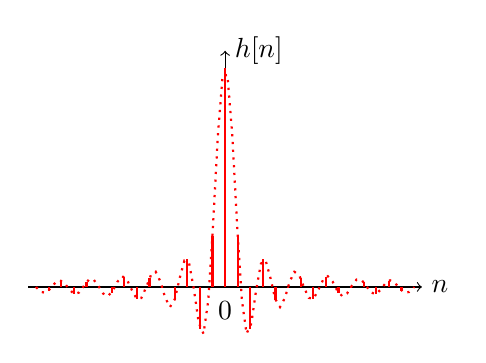
\begin{tikzpicture}
\draw[->] (-2.5,0)-- (2.5,0) node[right]{$n$};
\draw (0,-0.3) node {0};
\draw[->] (0,0)-- (0,3)node[right]{$h[n]$};

\draw[dotted,thick, domain=-2.4:2.4,color=red,samples=80] plot (\x,{160*sin(5*3.14*\x r  )/(5*3.14*\x r)});
\draw[thick, domain=-2.4:2.4,color=red,samples=31] plot [ycomb] (\x,{160*sin(5*3.14*\x r  )/(5*3.14*\x r)});


\end{tikzpicture}
\end{center}
\vspace{0.3cm}
\[ h[n] = \frac{\sin(\pi nT_e)}{\pi n T_e} \]

\end{columns}

\end{frame} 

\subsubsection{Réponse impulsionnelle réelle : fenêtrage}
\begin{frame}
\frametitle{Premier exemple :  Filtre passe-bas idéal} 
\textbf{PROBL\`EME !!!}

\begin{columns}
\column{60mm}
\begin{center}
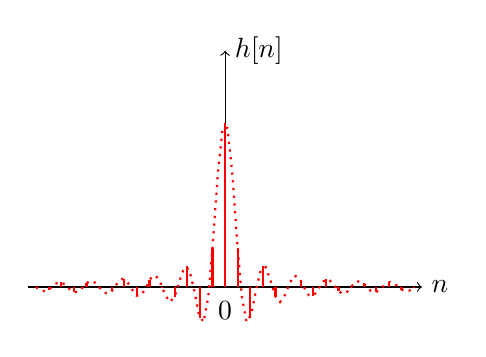
\begin{tikzpicture}
\draw[->] (-2.5,0)-- (2.5,0) node[right]{$n$};
\draw (0,-0.3) node {0};
\draw[->] (0,0)-- (0,3)node[right]{$h[n]$};

\draw[dotted,thick, domain=-2.4:2.4,color=red,samples=80] plot (\x,{120*sin(5*3.14*\x r  )/(5*3.14*\x r)});
\draw[thick, domain=-2.4:2.4,color=red,samples=31] plot [ycomb] (\x,{120*sin(5*3.14*\x r  )/(5*3.14*\x r)});


\end{tikzpicture}
\end{center}

\column{60mm}

\only<2->{
La réponse impulsionnelle est \textbf{infinie}\\
\vspace{1cm}

}

\only<3->{
On ne peut pas coder cette fonction sur un support numérique...
}

\end{columns}
\end{frame}

\begin{frame}
\frametitle{Premier exemple :  Filtre passe-bas idéal} 

\begin{columns}
\column{60mm}
\begin{center}
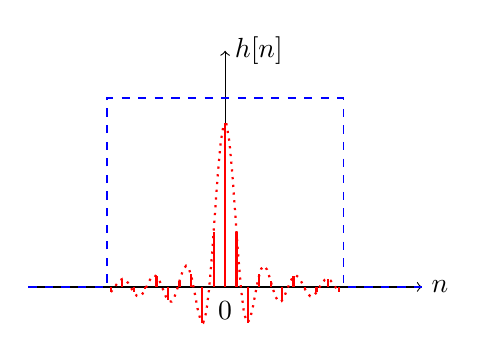
\begin{tikzpicture}
\draw[->] (-2.5,0)-- (2.5,0) node[right]{$n$};
\draw (0,-0.3) node {0};
\draw[->] (0,0)-- (0,3)node[right]{$h[n]$};

\draw[dotted,thick, domain=-1.45:1.45,color=red,samples=80] plot (\x,{120*sin(5*3.14*\x r  )/(5*3.14*\x r)});
\draw[thick, domain=-1.45:1.45,color=red,samples=21] plot [ycomb] (\x,{120*sin(5*3.14*\x r  )/(5*3.14*\x r)});

\only<2->{
		\draw[dashed,blue] (-2.5,0)--(-1.5,0)--(-1.5,2.4)--(1.5,2.4)--(1.5,0)--(2.5,0);
}


\end{tikzpicture}
\end{center}

\column{60mm}
Il faut un nombre \textbf{fini} d'échantillon\\
\vspace{1cm}
\only<2->{
$\rightarrow$ Application d'une \textbf{fenêtre temporelle}.
\\}
\vspace{1cm}
\only<3->{
Effet de l'application de la fenêtre sur la réponse en fréquence ?
}

\end{columns}
\end{frame}

\begin{frame}
\frametitle{Premier exemple :  Filtre passe-bas idéal} 

\begin{columns}
\column{50mm}
\begin{center}
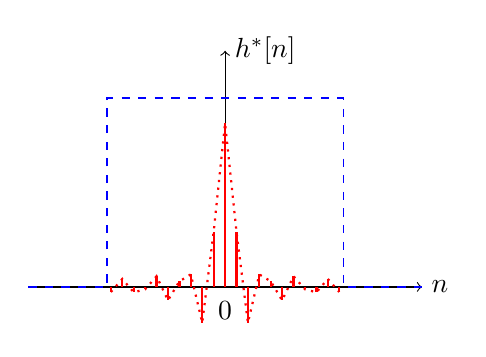
\begin{tikzpicture}
\draw[->] (-2.5,0)-- (2.5,0) node[right]{$n$};
\draw (0,-0.3) node {0};
\draw[->] (0,0)-- (0,3)node[right]{$h^*[n]$};

\draw[dotted,thick, domain=-1.45:1.45,color=red,samples=21] plot (\x,{120*sin(5*3.14*\x r  )/(5*3.14*\x r)});
\draw[thick, domain=-1.45:1.45,color=red,samples=21] plot [ycomb] (\x,{120*sin(5*3.14*\x r  )/(5*3.14*\x r)});


		\draw[dashed,blue] (-2.5,0)--(-1.5,0)--(-1.5,2.4)--(1.5,2.4)--(1.5,0)--(2.5,0);
\end{tikzpicture}
\end{center}

\column{70mm}

Effet de l'application de la fenêtre sur la réponse en fréquence ?\\
\vspace{0.5cm}
\[ h^*[n] = \frac{\sin(\pi nT_e)}{\pi n T_e}\cdot \Pi_M[n]  \]\\
\vspace{0.5cm}
\only<1>{\[ H^*(f) = ?  \]}
\only<2->{\[\boxed{ H^*(f) = TF(\frac{\sin(\pi nT_e)}{\pi n T_e}) \star TF(\Pi_M[n])}  \]}



\end{columns}
\end{frame}

\begin{frame}
\frametitle{Premier exemple :  Filtre passe-bas idéal} 

\begin{columns}[T]
\column{60mm}
\[h^*[n] = \frac{\sin(\pi nT_e)}{\pi n T_e}\cdot \Pi_M[n]\]\\
\vspace{0.5cm}
\begin{center}
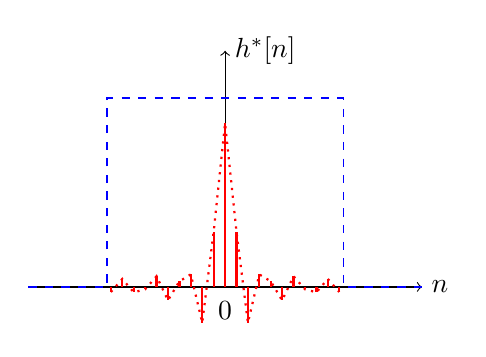
\begin{tikzpicture}
\draw[->] (-2.5,0)-- (2.5,0) node[right]{$n$};
\draw (0,-0.3) node {0};
\draw[->] (0,0)-- (0,3)node[right]{$h^*[n]$};

\draw[dotted,thick, domain=-1.45:1.45,color=red,samples=21] plot (\x,{120*sin(5*3.14*\x r  )/(5*3.14*\x r)});
\draw[thick, domain=-1.45:1.45,color=red,samples=21] plot [ycomb] (\x,{120*sin(5*3.14*\x r  )/(5*3.14*\x r)});


		\draw[dashed,blue] (-2.5,0)--(-1.5,0)--(-1.5,2.4)--(1.5,2.4)--(1.5,0)--(2.5,0);
\end{tikzpicture}
\end{center}

\column{60mm}
\[ H^*(f) = TF(\frac{\sin(\pi nT_e)}{\pi n T_e}) \star TF(\Pi_M[n]) \]\\
\vspace{0.3cm}
\begin{center}
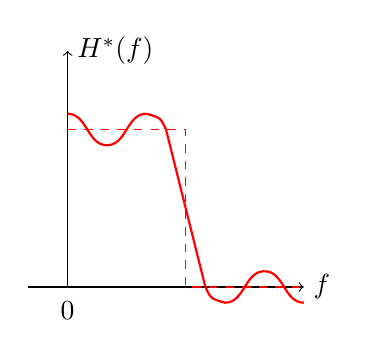
\begin{tikzpicture}

	\draw[->] (-0.5,0)-- (3,0)node[right] {$f$};
\draw (0,-0.3) node {0};
\draw[->] (0,0)-- (0,3) node[right] {$H^*(f)$};


\draw[dashed,red]   (0,2)--(1.5,2)--(1.5,0)--(3,0);

%ondulations BP
 \draw[thick,red] (0,2.2) .. controls (0.25,2.2)  and (0.25,1.8)  .. (0.5,1.8);
  \draw[thick,red] (0.5,1.8) .. controls (0.75,1.8)  and (0.75,2.2)  .. (1,2.2);
   \draw[thick,red] (1,2.2) .. controls (1.18,2.15) and (1.18,2.15)  .. (1.25,2);


%(1.5,2.1) and (1.2,2.1) 

%droite descendant de 1 à 0
\draw[thick,red] (1.25,2)--(1.75,0);

%ondulations BA
  \draw[thick,red] (2,-0.2) .. controls (2.25,-0.2)  and (2.25,0.2)  .. (2.5,0.2);
 \draw[thick,red] (2.5,0.2) .. controls (2.75,0.2)  and (2.75,-0.2)  .. (3,-0.2);
    \draw[thick,red] (1.75,0) .. controls (1.82,-0.15) and (1.82,-0.15)  .. (2,-0.2);


\end{tikzpicture}
\end{center}

\end{columns}

\begin{block}{}
Limitation du nombre de termes $\rightarrow$  Ondulations dans la fonction de transfert
\end{block}

\end{frame}

\begin{frame}
\frametitle{Premier exemple :  Filtre passe-bas idéal} 

\begin{columns}[T]
\column{45mm}
\begin{center}
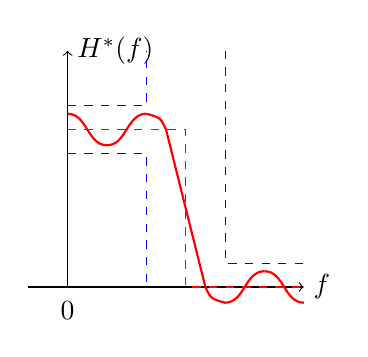
\begin{tikzpicture}

	\draw[->] (-0.5,0)-- (3,0)node[right] {$f$};
\draw (0,-0.3) node {0};
\draw[->] (0,0)-- (0,3) node[right] {$H^*(f)$};


\draw[dashed,red]   (0,2)--(1.5,2)--(1.5,0)--(3,0);

%ondulations BP
 \draw[thick,red] (0,2.2) .. controls (0.25,2.2)  and (0.25,1.8)  .. (0.5,1.8);
  \draw[thick,red] (0.5,1.8) .. controls (0.75,1.8)  and (0.75,2.2)  .. (1,2.2);
   \draw[thick,red] (1,2.2) .. controls (1.18,2.15) and (1.18,2.15)  .. (1.25,2);


%(1.5,2.1) and (1.2,2.1) 

%droite descendant de 1 à 0
\draw[thick,red] (1.25,2)--(1.75,0);
    \only<2->{
		
\draw[dashed,blue](0,1.7)--(1,1.7)--(1,0);
\draw[dashed,blue](0,2.3)--(1,2.3)--(1,3);
\draw[dashed,blue](2,3)--(2,0.3)--(3,0.3);
}   
%ondulations BA
  \draw[thick,red] (2,-0.2) .. controls (2.25,-0.2)  and (2.25,0.2)  .. (2.5,0.2);
 \draw[thick,red] (2.5,0.2) .. controls (2.75,0.2)  and (2.75,-0.2)  .. (3,-0.2);
    \draw[thick,red] (1.75,0) .. controls (1.82,-0.15) and (1.82,-0.15)  .. (2,-0.2);
    
%    \only<2->{
%		
%\draw[dashed,blue](0,1.7)--(1,1.7)--(1,0);
%\draw[dashed,blue](0,2.3)--(1,2.3)--(1,3);
%\draw[dashed,blue](2,3)--(2,0.3)--(3,0.3);
%}    
    
    \end{tikzpicture}
\end{center}


\column{75mm}
On résume :
\begin{itemize}
\item<2-> Réponse impulsionnelle du passe-bas idéal ? \only<3->{ sinus cardinal discret (nombre infini de terme)}
\vspace{0.3cm}
\item<4-> Nombre fini de termes rép. imp. $\rightarrow$ application d'une fenêtre rectangulaire
\vspace{0.3cm}
\item<5-> Fenêtrage en temporel $\rightarrow$ Ondulations sur la fonction  de transfert du filtre réel

\end{itemize}
\end{columns}

\end{frame}

\begin{frame}
\frametitle{Premier exemple :  Filtre passe-bas idéal} 
Reprenons le gabarit...
\begin{columns}[T]
\column{45mm}
\begin{center}
\begin{tikzpicture}

	\draw[->] (-0.5,0)-- (3,0)node[right] {$f$};
\draw (0,-0.5) node {0};
\draw[->] (0,0)-- (0,3) node[right] {$H^*(f)$};


\draw[dashed,red]   (0,2)--(1.5,2)--(1.5,0)--(3,0);

%ondulations BP
 \draw[thick,red] (0,2.2) .. controls (0.25,2.2)  and (0.25,1.8)  .. (0.5,1.8);
  \draw[thick,red] (0.5,1.8) .. controls (0.75,1.8)  and (0.75,2.2)  .. (1,2.2);
   \draw[thick,red] (1,2.2) .. controls (1.18,2.15) and (1.18,2.15)  .. (1.25,2);


%(1.5,2.1) and (1.2,2.1) 

%droite descendant de 1 à 0
\draw[thick,red] (1.25,2)--(1.75,0);
    \only<2->{
		
\draw[dashed,blue](0,1.7)--(1,1.7)--(1,0);
\draw[dashed,blue](0,2.3)--(1,2.3)--(1,3);
\draw[dashed,blue](2,3)--(2,0.3)--(3,0.3);
}   
%ondulations BA
  \draw[thick,red] (2,-0.2) .. controls (2.25,-0.2)  and (2.25,0.2)  .. (2.5,0.2);
 \draw[thick,red] (2.5,0.2) .. controls (2.75,0.2)  and (2.75,-0.2)  .. (3,-0.2);
    \draw[thick,red] (1.75,0) .. controls (1.82,-0.15) and (1.82,-0.15)  .. (2,-0.2);
    
    \only<2->{
		
\draw[dashed,blue](0,1.7)--(1,1.7)--(1,0);
\draw[dashed,blue](0,2.3)--(1,2.3)--(1,3);
\draw[dashed,blue](2,3)--(2,0.3)--(3,0.3);
}    
\only<4->{
\draw (1,-0.5) node {$f_1$};
\draw (2,-0.5) node {$f_2$};
\draw (-0.6,1.7) node {$1 - \delta_1$};
\draw (-0.6,2.3) node {$1 + \delta_1$};
\draw (-0.3,0.4) node {$\delta_2$};
}
    \end{tikzpicture}
\end{center}


\column{75mm}
Commentaires:
\begin{itemize}
\item<3-> filtre réel (nombre fini de termes) = \textbf{Oscillations rép. en fréq.}
\vspace{0.3cm}
\item<4-> Oscillations = tolérance en amplitude + largeur de transition
\vspace{0.3cm}
\item<5-> + de termes = - d'oscillations MAIS mémoire et temps de calcul à prendre en compte
\end{itemize}
\end{columns}

\end{frame}

\subsection{Synthèse de filtres non-récursifs: Méthode des fenêtres}

\begin{frame}
\frametitle{Synthèse de filtres non-récursifs: Méthode des fenêtres}

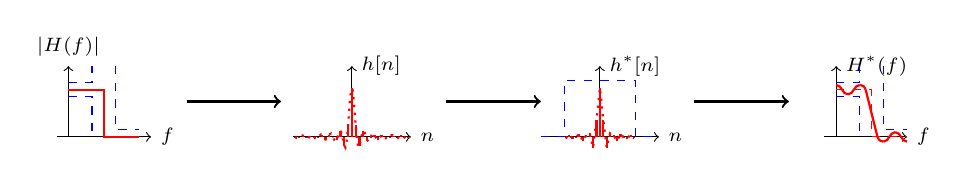
\begin{tikzpicture}
\begin{scope}[scale=0.3]
	\draw[->] (-0.5,0)-- (3.5,0)node[right] {\scriptsize $f$} ;
%\draw (-0.3,-0.3) node {0};
\draw[->] (0,0)-- (0,3)node[above] {\scriptsize $|H(f)|$};


%\draw (3,-0.3) node {$f_e/2$};


\draw[dashed,blue](0,1.7)--(1,1.7)--(1,0);
\draw[dashed,blue](0,2.3)--(1,2.3)--(1,3);
\draw[dashed,blue](2,3)--(2,0.3)--(3,0.3);

	\draw[thick,red]   (0,2)--(1.5,2)--(1.5,0)--(3,0);
	%\draw[->,thick] (0.75,-0.5)--(0.75,-1);
	%\draw (1.5,-0.3) node {$f_e/4$};
	\draw[->,thick] (5,1.5)--(9,1.5);
\end{scope}



\begin{scope}[scale=0.3,xshift=12cm]
%\draw[->,thick] (0,4)--(0,3.4);
\draw[->] (-2.5,0)-- (2.5,0) node[right]{\scriptsize $n$};
%\draw (0,-0.3) node {0};
\draw[->] (0,0)-- (0,3)node[right]{\scriptsize $h[n]$};

\draw[dotted,thick, domain=-2.4:2.4,color=red,samples=80] plot (\x,{120*sin(5*3.14*\x r  )/(5*3.14*\x r)});
\draw[thick, domain=-2.4:2.4,color=red,samples=31] plot [ycomb] (\x,{120*sin(5*3.14*\x r  )/(5*3.14*\x r)});
\draw[->,thick] (4,1.5)--(8,1.5);
\end{scope} 



\begin{scope}[scale=0.3,xshift=22.5cm]
\draw[->] (-2.5,0)-- (2.5,0) node[right]{\scriptsize $n$};
%\draw (0,-0.3) node {0};
\draw[->] (0,0)-- (0,3)node[right]{\scriptsize $h^*[n]$};

\draw[dotted,thick, domain=-1.45:1.45,color=red,samples=21] plot (\x,{120*sin(5*3.14*\x r  )/(5*3.14*\x r)});
\draw[thick, domain=-1.45:1.45,color=red,samples=21] plot [ycomb] (\x,{120*sin(5*3.14*\x r  )/(5*3.14*\x r)});


		\draw[dashed,blue] (-2.5,0)--(-1.5,0)--(-1.5,2.4)--(1.5,2.4)--(1.5,0)--(2.5,0);
		
		\draw[->,thick] (4,1.5)--(8,1.5);
		\end{scope}
		
		%\draw[->,thick] (26,1)--(31,1);
		
		\begin{scope}[scale=0.3,xshift=32.5cm]
	\draw[->] (-0.5,0)-- (3,0)node[right] {\scriptsize $f$};
%\draw (0,-0.5) node {0};
\draw[->] (0,0)-- (0,3) node[right] {\scriptsize $H^*(f)$};


\draw[dashed,red]   (0,2)--(1.5,2)--(1.5,0)--(3,0);

%ondulations BP
 \draw[thick,red] (0,2.2) .. controls (0.25,2.2)  and (0.25,1.8)  .. (0.5,1.8);
  \draw[thick,red] (0.5,1.8) .. controls (0.75,1.8)  and (0.75,2.2)  .. (1,2.2);
   \draw[thick,red] (1,2.2) .. controls (1.18,2.15) and (1.18,2.15)  .. (1.25,2);


%(1.5,2.1) and (1.2,2.1) 

%droite descendant de 1 à 0
\draw[thick,red] (1.25,2)--(1.75,0);
  
\draw[dashed,blue](0,1.7)--(1,1.7)--(1,0);
\draw[dashed,blue](0,2.3)--(1,2.3)--(1,3);
\draw[dashed,blue](2,3)--(2,0.3)--(3,0.3);
 
%ondulations BA
  \draw[thick,red] (2,-0.2) .. controls (2.25,-0.2)  and (2.25,0.2)  .. (2.5,0.2);
 \draw[thick,red] (2.5,0.2) .. controls (2.75,0.2)  and (2.75,-0.2)  .. (3,-0.2);
    \draw[thick,red] (1.75,0) .. controls (1.82,-0.15) and (1.82,-0.15)  .. (2,-0.2);
    
\end{scope}
	

\end{tikzpicture}\\
\vspace{0.5cm}
\textbf{Méthodes de fenêtres} :\\
\vspace{0.2cm}
\begin{enumerate}
\item Réponse en fréquence de filtre idéal 
\vspace{0.2cm}
\item<2-> Réponse impulsionnelle idéale 
\vspace{0.2cm}
\item<3-> Fenêtrage $\rightarrow$ réponse impulsionnelle réelle 
\vspace{0.2cm}
\item<4-> Réponse en fréquence réelle
\end{enumerate}



\end{frame}

\begin{frame}
\frametitle{Synthèse de filtres non-récursifs: Méthode des fenêtres}

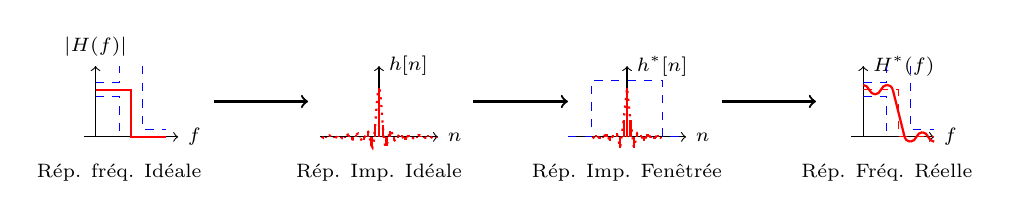
\begin{tikzpicture}
\begin{scope}[scale=0.3]
	\draw[->] (-0.5,0)-- (3.5,0)node[right] {\scriptsize $f$} ;
%\draw (-0.3,-0.3) node {0};
\draw[->] (0,0)-- (0,3)node[above] {\scriptsize $|H(f)|$};


%\draw (3,-0.3) node {$f_e/2$};


\draw[dashed,blue](0,1.7)--(1,1.7)--(1,0);
\draw[dashed,blue](0,2.3)--(1,2.3)--(1,3);
\draw[dashed,blue](2,3)--(2,0.3)--(3,0.3);

	\draw[thick,red]   (0,2)--(1.5,2)--(1.5,0)--(3,0);
	%\draw[->,thick] (0.75,-0.5)--(0.75,-1);
	%\draw (1.5,-0.3) node {$f_e/4$};
	\draw[->,thick] (5,1.5)--(9,1.5);
	\draw (1,-1.5) node[text centered] {\scriptsize Rép. fréq. Idéale};
\end{scope}



\begin{scope}[scale=0.3,xshift=12cm]
%\draw[->,thick] (0,4)--(0,3.4);
\draw[->] (-2.5,0)-- (2.5,0) node[right]{\scriptsize $n$};
%\draw (0,-0.3) node {0};
\draw[->] (0,0)-- (0,3)node[right]{\scriptsize $h[n]$};

\draw[dotted,thick, domain=-2.4:2.4,color=red,samples=80] plot (\x,{120*sin(5*3.14*\x r  )/(5*3.14*\x r)});
\draw[thick, domain=-2.4:2.4,color=red,samples=31] plot [ycomb] (\x,{120*sin(5*3.14*\x r  )/(5*3.14*\x r)});
\draw[->,thick] (4,1.5)--(8,1.5);
	\draw (0,-1.5) node[text centered] {\scriptsize Rép. Imp. Idéale};
\end{scope} 



\begin{scope}[scale=0.3,xshift=22.5cm]
\draw[->] (-2.5,0)-- (2.5,0) node[right]{\scriptsize $n$};
%\draw (0,-0.3) node {0};
\draw[->] (0,0)-- (0,3)node[right]{\scriptsize $h^*[n]$};

\draw[dotted,thick, domain=-1.45:1.45,color=red,samples=21] plot (\x,{120*sin(5*3.14*\x r  )/(5*3.14*\x r)});
\draw[thick, domain=-1.45:1.45,color=red,samples=21] plot [ycomb] (\x,{120*sin(5*3.14*\x r  )/(5*3.14*\x r)});


		\draw[dashed,blue] (-2.5,0)--(-1.5,0)--(-1.5,2.4)--(1.5,2.4)--(1.5,0)--(2.5,0);
		
		\draw[->,thick] (4,1.5)--(8,1.5);
			\draw (0,-1.5) node[text centered] {\scriptsize Rép. Imp. Fenêtrée};
		\end{scope}
		
		%\draw[->,thick] (26,1)--(31,1);
		
		\begin{scope}[scale=0.3,xshift=32.5cm]
	\draw[->] (-0.5,0)-- (3,0)node[right] {\scriptsize $f$};
%\draw (0,-0.5) node {0};
\draw[->] (0,0)-- (0,3) node[right] {\scriptsize $H^*(f)$};


\draw[dashed,red]   (0,2)--(1.5,2)--(1.5,0)--(3,0);

%ondulations BP
 \draw[thick,red] (0,2.2) .. controls (0.25,2.2)  and (0.25,1.8)  .. (0.5,1.8);
  \draw[thick,red] (0.5,1.8) .. controls (0.75,1.8)  and (0.75,2.2)  .. (1,2.2);
   \draw[thick,red] (1,2.2) .. controls (1.18,2.15) and (1.18,2.15)  .. (1.25,2);


%(1.5,2.1) and (1.2,2.1) 

%droite descendant de 1 à 0
\draw[thick,red] (1.25,2)--(1.75,0);
  
\draw[dashed,blue](0,1.7)--(1,1.7)--(1,0);
\draw[dashed,blue](0,2.3)--(1,2.3)--(1,3);
\draw[dashed,blue](2,3)--(2,0.3)--(3,0.3);
 
%ondulations BA
  \draw[thick,red] (2,-0.2) .. controls (2.25,-0.2)  and (2.25,0.2)  .. (2.5,0.2);
 \draw[thick,red] (2.5,0.2) .. controls (2.75,0.2)  and (2.75,-0.2)  .. (3,-0.2);
    \draw[thick,red] (1.75,0) .. controls (1.82,-0.15) and (1.82,-0.15)  .. (2,-0.2);
    \draw (1,-1.5) node[text centered] {\scriptsize Rép. Fréq. Réelle};
\end{scope}
	

\end{tikzpicture}\\
\vspace{0.5cm}
\textbf{Remarques} :\\
\vspace{0.2cm}
\begin{itemize}
\item Plusieurs fenêtres sont possibles (Hamming, Dolf Tchebycheff,...)
\vspace{0.2cm}
\item<2-> Fenêtre $\rightarrow$ Compromis ondulations/largeur bande de transition
\vspace{0.2cm}
\item<3-> Faible largeur transition = Ondulations importantes 
\vspace{0.2cm}
\item<4-> Méthode assez directe mais pas forcément optimale... 
\end{itemize}

\end{frame}

\subsection{Synthèse de filtres non-récursifs: Différentes méthodes}
\begin{frame}
\frametitle{Synthèse de filtres non-récursifs: Différentes méthodes}
Les méthodes suivent toute le même principe général :

\begin{center}
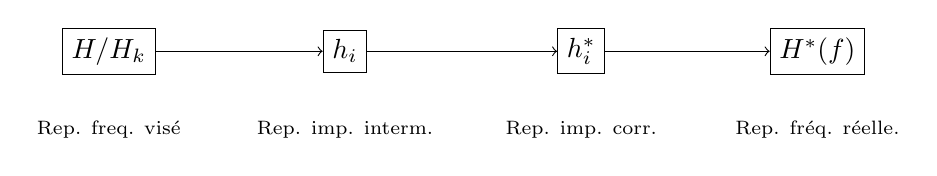
\begin{tikzpicture}
		\node[rectangle,draw,align=center] (I) at (1,0) {$H/H_k$};
		\draw (1,-1) node[text centered] {\scriptsize Rep. freq. visé};
		\node[rectangle,draw,align=center] (D) at (4,0) {$h_i$};
		\draw (4,-1) node[text centered] {\scriptsize Rep. imp. interm.};
		\node[rectangle,draw,align=center] (N) at (7,0) {$h_i^*$};
				\draw (7,-1) node[text centered] {\scriptsize Rep. imp. corr.};
		\node[rectangle,draw,align=center] (B) at (10,0) {$H^*(f)$};	
		\draw (10,-1) node[text centered]{\scriptsize Rep. fréq. réelle.};
		
		\draw[->] (I)--(D);
		\draw[->] (D)--(N);
		\draw[->] (N)--(B);
\end{tikzpicture}
\end{center}

Principales méthodes de synthèse de filtres non-récursifs:
\vspace{0.2cm}
\begin{itemize}
\item<2-> Méthode des fenêtres 
\item<3-> Méthode de l'échantillonnage en fréquence
\item<4-> Méthode des moindres carrés
\item<5-> Méthode par approximation de Tchebychev
\end{itemize}

\end{frame}

\subsection{Méthode de l'échantillonnage en fréquence}

\end{document}